\hypertarget{disobedient-action-research-cycles}{%
\section{Disobedient Action Research
Cycles}\label{disobedient-action-research-cycles}}

This chapter follows on from the framing of the last two chapters to
discuss how I have formed a methodology for this research project. The
methodology I have taken up is a situated implementation of disobedient
action research. This disobedience and its foundations of action
research follows the many crip and queer figures that were called on in
the last chapter, and especially within
\href{../../01_Disability_justice_and_life_affirmation_flipping_the_table/sections/01.02.04_Cripping_Technoscience.md}{01.02.04\_Cripping\_Technoscience},
where it demands to step out of line, to find other routes that
institutional inflexibilities do not have the capacity for and to
defiantly take those actions now.

In this move to shake off the the academic table of methods that holds
us in-line, I turned to action research as a place to empower the
position of practitioners (in this case collaborators and I) as a
knowledge creators. This methodology approaches these experiences by
giving depth and insight to relations where an embodied framing makes
room for it to be understood in action, from a situated perspective and
knowledge. I then move to orient this methodology through first person
action research, where I bring in the background of my research and to
make room within it for a situated embodiment of these inquiries. From
this position and that of my crip framing, I felt this research
necessitates a disobedient approach, one that manifests a disorientation
of the scope and norms of the actions within action research. It poses
this work to take on direct actions together right now! Of refusing to
be a part of, assimilate to and be quiet about certain politics and
their violent relations!

After this setting up of a disobedient action research methodology I go
on to discuss how I have taken up this methodology in three (ish) cycles
of action and reflection, and how they have been approached at different
intersections of social and technical infrastructures within and around
institutions.

\hypertarget{action-research}{%
\subsection{Action research}\label{action-research}}

This section brings into focus why this research has oriented towards
action research as a methodology. Following on from the
\href{../../01_Disability_justice_and_life_affirmation_flipping_the_table/01_Disability\%20justice\%20and\%20life\%20affirmation\%20flipping\%20the\%20table.md}{01\_Disability
justice and life affirmation flipping the table} chapter and its framing
of embodied and relational politics I have found that action research
aligns and intersects at a number of places that are key. To trace these
crossing lines I am working with Judi Marshall's notion of Living Life
as Inquiry (LLI) (Gearty and Marshall 2021; Marshall 1999) and Living
Systemic Thinking (Marshall 2004) that make room for me to not only take
on the calls for action I have made in the previous chapter but also to
bring into those actions the necessary reflection that quality inquiry
and research entails\footnote{``quality (a term I prefer to
  `validity')'' - marshal living systemic}.

Marshall's LLI (1999; 2004; Gearty and Marshall 2021) work is a specific
type of action research named first person action research, which is
where the first intersection crosses paths with my proposed framework.
In first person action research Marshall is in many ways practicing a
methodology that makes room for the background of the practitioner to
settle in, like Ahmed (2006), and brings in the context, relations and
feelings of the person making the research. In her essay \emph{Living
Life as Inquiry -- a Systemic Practice for Change Agents (2021)} with
Margaret Rose Gearty, which acts as a 20 year celebration and
retrospective since the paper and method was first published and to
examine how LLI has been taken up in many orientations. There are a
number of focuses in this essay on how \emph{Living Life as Inquiry} can
be practised but there is a key focus on how it makes room for an
embodiment of research. Marshall phrases it as ``Inquiry has woven
itself into my life'' (2021, 454). This embodiment and weaving of
research into life is key for my practice as it makes room for me to
wiggle into this research, my experiences of being crip and queer within
and around institutional limits and their relations. It let's me situate
this research to my context, to think through what it means for me as a
middle class `white', crip and queer researcher, with chronic illness,
pain and fatigue to be approaching deeply neo-liberal and efficiency
driven institutions in the UK. This embodiment of research also enables
me to think about how these positions of practice and of making embodied
actions is itself a space of knowledge generation, and one that finds
the capture or determination of these knowledges impossible in many
ways. In Living Systemic Thinking (2004) Marshall gives the example of
her colleagues and her reflecting on a review process of a student, to a
fine grain of reflection, and shows how each person interprets these
relations differently. She approaches this not to de-validate the
difference and nuance but to work with these varied perspectives as
other orientations of an issue, that form their own understandings of
these actions and their relations to them (ibid, 15). Marshall's
position on the embodiment of research also offers me to bring feelings
and affect into practice, intersecting with a crip focus on affectivity.
This navigation of embodiment informs my orientation of actions and
their deliberation to not be led by but to account for how it has felt
within the relations, how what is expected causes friction or how what I
desire to undertake brings joy.

With this engagement of self, of bringing feelings into action, and
those actions into inquiry and knowing they pose another way of
orienting myself. Marshall and Gearty through their approach to LLI also
ask of me to think about how I direct or orient myself, much like I
discussed in the
\href{../../01_Disability_justice_and_life_affirmation_flipping_the_table/sections/01.01.00_Orienting_the_table.md}{01.01.00\_Orienting\_the\_table}
section through the work of Ahmed. With LLI they think through how these
practitioner and actioned knowledges that I practice, can in themselves
form alternative orientations to those of hegemony and institutions. In
an essay called \emph{Living Systemic Thinking} (ibid) Marshall terms it
as ``sense making'', and later on her and Gearty ask us to work with
this sensing think through ``when to persist or desist'' (2021, 457) in
direction. With this they present Living Life as Inquiry as a method to
process what to inquire into and how to orient relational actions
towards that outcome. To do this in this embodied context they work with
a few notions to consider how to feel out what is appropriate to be done
in that context. They talk about ``staying fresh and open'' (ibid, 455),
where by taking life into inquiry, we question our habits, our
sedimented patterns and norms to think through and feel out other
approaches and paths to the outcome. To do this they propose ``checking
for signs of vitality'' (ibid, 455) as a way to do pulse-checks, to ask
``How am I, here and now?'', and to balance between inquiring mindlessly
forward and being stuck within the fine grain and frozen. They also pose
these pulse-checks to be embodied and not always consciously reasoned to
aim to unravel the notion of ``pursuit'' within research. This is where
I can move away from a determined end goal or sedimented straight path
and tending towards feeling out dynamic and emerging research to decide
the next actions to make. They also bring up the notion of ``working
with emotions''( ibid, 456) as a way to inquire into ``what is really
important'', of connecting to the issue on an embodied level and letting
these feelings not determine but be engaged in what I feel I need to
tend to.

This leads onto their proposition of ``practices of discernment'' (ibid,
457), which interestingly isn't about where to act but more about when.
As they note it can be about discerning when to be ``waiting things
out'' and when to be working out ``what is what'' before deciding how to
act, positioning Marshall's notion on ``when to persist or desist''
within time. Practising this within Ahmed's framing of inherited and
sedimented relations makes room for me to think, where am I now, and
what can I change within my reach. In a textural response to this notion
Marshall and Gearty give the image of the Heron/yoga pose, of one leg in
the water, of feeling the ripples and many forms of data lap against
your body and to patiently discern what they mean and what/when to
action. They follow this texture with their notion of ``the timely move
to action'' (ibid, 458), which continues to ask how and when to take
actions of inquiry but also where. In this embodied methodology they
prompt us to think through where this can be in the relations we are
entangled into, which can be an internal action on the self, or an
``inward action'' as they term it. In doing this though they don't
divide between what they call the inward and outward arcs of action, but
instead see them as performances of an entangled process. This prompts
this research to re-scope where the actions of action research can be
taken when embodied in research, and has pushed me as a practitioner to
inquire into how I am internally orienting practices and how this is
affected by and affecting outward actions.

Following on from (but also maybe before/during) is their conception of
reflection of action. Why I say maybe before/during is due to the
troubling of the separation of action and reflection that LLI
encourages. Instead with LLI Marshall and Gearty ask me to be open to
the complex ways that these movements of action and reflection are
entwined and interdependent, with reflection being in many ways an
action in itself. Within this dialogue of reflection in mind they form
another few notions to think with and help reflect on what matters
within and around our actions. They ask us to revisit the ``inner and
outer arcs of attention'' (ibid, 458), and that by taking time with both
the internal embodied and external actions each will inform and develop
the understanding of one another. Somewhat intersecting with crip theory
they compare the entanglement of these arcs to that of the bodymind, and
its move to dissolve the boundary between the two, where action and
reflection move as one muscle. This is also closely read into in
\emph{Living Systemic Thinking (2004)} where Marshall takes up a close
reading and reflection of their approach at each stage in line with
feedback from colleagues to deliver a quality emerging inquiry into
institutional processes through her enactment and relation to them.

Returning to LLI they also work with the notion of ``the processual
nature of inquiry'' (ibid, 459) that prompts us to approach these cycles
of sense-making as ways to move beyond the determined and inherited
generalised models of research and instead situate these orientating
processes within the embodied practices of the researcher. In these
modes of orienting they pose knowledge as ephemeral and fleeting as it
sits within the relation of action and practice. They open to reflection
that does not model, generalise and predetermine moments but evoke
practice that makes room for me to visit the relations I engage in
afresh to rethink the sedimented paths we take towards them. In this
move and throughout the paper they also open up to what they call
\emph{textures}, such as the Heron description above, which takes the
form of images, figures and reflections that act as experiments of how
to express these feelings, practices and enquires where words may fail
us. This orientation of modes of reflection within Action Research
intersects well with a crip position, and one which I relate to a lot,
where words can escape me. Here they make room for these discursive
knowledges through embodied technical and social practices to be
validated as generative ways of getting to know the relational
``problems'' at hand through other revealing practices. How drawing,
metaphoring and coding can be ways to reflect and key modes of action,
inquiry and sense-making. The last notion they leave us with is that of
``reviewing generative/degenerative aspects of inquiry'' (2021, 459),
and is a very kind one that in many ways echo's that of pulse-checking.
With this notion they discuss the balance you have to take in
first-person inquiry to not get caught in self-critical cycles, which
can stop actions from taking place and trap researchers inward. To
manage this line they say to monitor what is being looked at, with
degenerative inquiry being characterised by ``over-rumination or
joylessness''. Here again aligning with a crip move to imagine
disalignment as a generative site, and one where there is always a
possibility of joy and pleasure. This is again where in places within
myself and in relation to others, we can inquire into how these sites of
friction as not invalidated and determined actions of humiliation, pain
and duress, but how they make room for the possibility to be joyous and
pleasurable places of inquiry.

Bringing LLI into action in this research has empowered me undertaking
it in a number of ways. It has made room for me to unfold and situate
the research within my manys contexts and practices as a crip and queer
researcher throughout the PhD. It has also prompted me to engage my
feelings, bodily relations and emotions into an embodied research
practice. It has given space to the technical and social practices I
undertake, of thinking through code, finding frictions in coalition and
of trying to survive within and around these institutions, as generative
and informative textures of this research. It has also buffered these
crip and queer notions of finding our own paths together, and that those
are ones we desire, find vital and map to our bodies. In retrospect
first person inquiry has given my research practice the capacity to
change paths. For example a key turning point in this research is that
through quality inquiry I decided to desist working with and for certain
logics of automation and organisation that invoke and determine
dominative centralised control and come from violent ableist and
eugenics histories. Instead to step back, reorient and persist at the
practice of social infrastructure that inform how to decentralise and
disorient their technical counterpart through community interdependence
and critical access.

In this move to desist to then persist I found though that there were
some crip frictions I have with this framing of LLI and Action Research
here. Even though they counter narratives of pursuit and make rooms for
finding my own way through embodied practices, their focus can be
somewhat be Cripped more in relation to instituional processes. When
Marshall references Meyerson and Scully's concept of ``tempered
radicals'' (1999, 3) it is hard to imagine crip theory so normalised,
subdued and conformed. Of course we get ``heated up and cooled down''
when ``being simultaneously outsider and insider'' of institutions, but
it is not about getting ``tougher''. I know that in my inquiry I have
moved, sometimes without reason from being tempered, to flexible, to
brittle, to wet, to rusted, to loose and to tempered again. This isn't
to say this divergence isn't possible within First Person AR, but the
Crip orientation I desire aims to move beyond the need to be tempered
towards institutional norms and our manifestings, as being tempered may
make unlivable the many approaches to a crip notion of justice and
radical access before they even begin. This is not to say being tempered
and playing the valid role of ``user'' or ``expert'' to subvert or hack,
or to reflect on the ways we emerge in relation to institutions are not
valid in this critique. It is instead to disorient this table of action
and to make known-able through critical access, the labours and their
knowledges that these institutions invalidate. In relation to my
experiences from and orientation to institutions and their imaginary
possibility for these radical politics and social relations we call for
is that they are limited through very restrictive terms that
collectively in my collaborations, we can only form small amounts of
wiggle room within and around. To find the space and relations that I
desire and that can start to make room for these sorts of imaginary
practices I turned disobediently from methods where I have to be
tempered, and I have disoriented this through crip theory,
interdependence and of movement making. This isn't to neglect the change
I can and have made in the institution, but it is to pivot from crip
futures they cannot hold. It is to make time and room to feel out my
orientation towards these more restrictive and sedimented organisational
practices of institutions, and figure out how to counter them.

\hypertarget{why-not-other-action-research}{%
\subsection{Why not other action
research?}\label{why-not-other-action-research}}

It is of course sensible to ask, and for me to reason why I have decided
on First Person Action Research instead of other modes of AR. This is
specifically true when it comes to Crip studies where the sedimented
path into action research would be through participatory research. A
quality example of this, and similarly to my research is the blurring of
the lines of community and institution is Laura J. Wernick's
\emph{Learning Disability Justice through Critical Participatory Action
Research} (2023). With this work she focuses on the notion of
participatory to surface the ways that disabled interdependence is what
has made her research happen. She also reflects on these exchanges in a
very embodied, vulnerable and situated approach that a Crip studies
approach encourages. This embodied mode being one that also crosses
heavily into First Person Action Research. In my research I have
similarly manifested it through these Crip support networks, through
interdependence and from community, and I definitely do not want to
underplay their participation in this work. I do though chose to orient
towards First Person Action Research as I want to focus not so much on
disabled people participating in the institutional norms or within
disabled exclusive space, but instead towards how crip people as active
change makers can transform the more intersectional organisations,
institutions and systems around us. In this move putting pressure on,
making friction with and giving feedback to the ableist institutions and
relations we are in-touch with. This again isn't to say that the work
like Wernick's that practice Participatory AR methods are not in reach
of this change on their bodily horizon, but it is to instead orient
towards this, and see how this imposition can change relations and
politics around us.

\hypertarget{disobedient-action-research}{%
\subsection{Disobedient action
research}\label{disobedient-action-research}}

``This is how as a method it links to what we call''disobedient
action-research", it invokes and invites further remediations that can
go from the academic paper to the bug report, from the narrative to the
diagrammatic and from tool mis-use to in-terface re-design to the
dance-floor. It provides us with inscriptions, de-scriptions and
re-in-terpretations of a vocabulary that is developing all along."
(Rocha and Snelting 2017, 45)

This is the point when this first person action research becomes a
disobedient form of Action Research. This is because it makes room for
these practices to move away from and refuse the institutional and
hegemonic norms that a crip orientation of justice also refuses. Much
like the disobedient demand of the \emph{Crip Technoscience Manifesto}
which I work with, and moves to access through friction (Hamraie and
Fritsch 2019, 10), disobedient action poses us to take direct actions
now! It aims to form futures within and around institutes that can't
hold them yet, and defiantly practice politics that they are not ready
to imagine. In the essay `\emph{We Have Always Been Geohackers}' (2021)
by Helen Pritchard, Jara Rocha and Femke Snelting, they position the
methodology of Disobedient Action Research as a means to re-scope and
re-think how we practice questioning, maintaining and developing
sociotechnical systems and infrastructures. As they pose it through this
essay, what does it mean to debug a system in the context of computing,
its institutions and politics that hold it in place. In the contexts and
configurations of their interventions, they ask how normative/obedient
debugging in open source communities often reinforces systems instead of
questioning and transforming them. Through their analysis they focus on
how breaking up the ``hardest problems'' into ``tiny'' and
``squeezable'' bugs can limit what can be said and done. This question
can also be easily applied through crip studies, where we could ask how
does fitting into and assimilating to the institution's ``squeezable''
terms of access actually limit the contingent possibilities of change we
could make otherwise?

In their essay they take up the debugging of Gplates, a free software
tool and web-portal for tectonic plate modelling and mineral prediction
for extraction. This debugging took place in a collective workshop where
a group of non-technocrats, nor technical specialists produced their own
independent knowledge, expertise and critiques of how these systems
figure tectonic movements and their volumetric predictions of mineral
resources. Through these non-hegemonic counter figures, the group
questioned the naturalised aesthetics and navigational tools of Gplates.
This includes questioning the representations of the globe's default as
a blank grey orb awaiting to be projected on us by the god like viewer
(\cref{fig:grey}), reinforced through to the time slider that lets you
smoothly slide through ``mega-annums of geological time'' (ibid, 250).
In questioning the software through these actions and reflections, they
open up conversations of what agencies does the earth, and those bodies
living on it have (ibid, 252-53). When a software has tool names
orientating ``grabbing'', especially around land, minerals and bodies,
what semantics, meaning and use does this inscribe (ibid, 252).

\begin{figure}
\hypertarget{fig:grey}{%
\centering
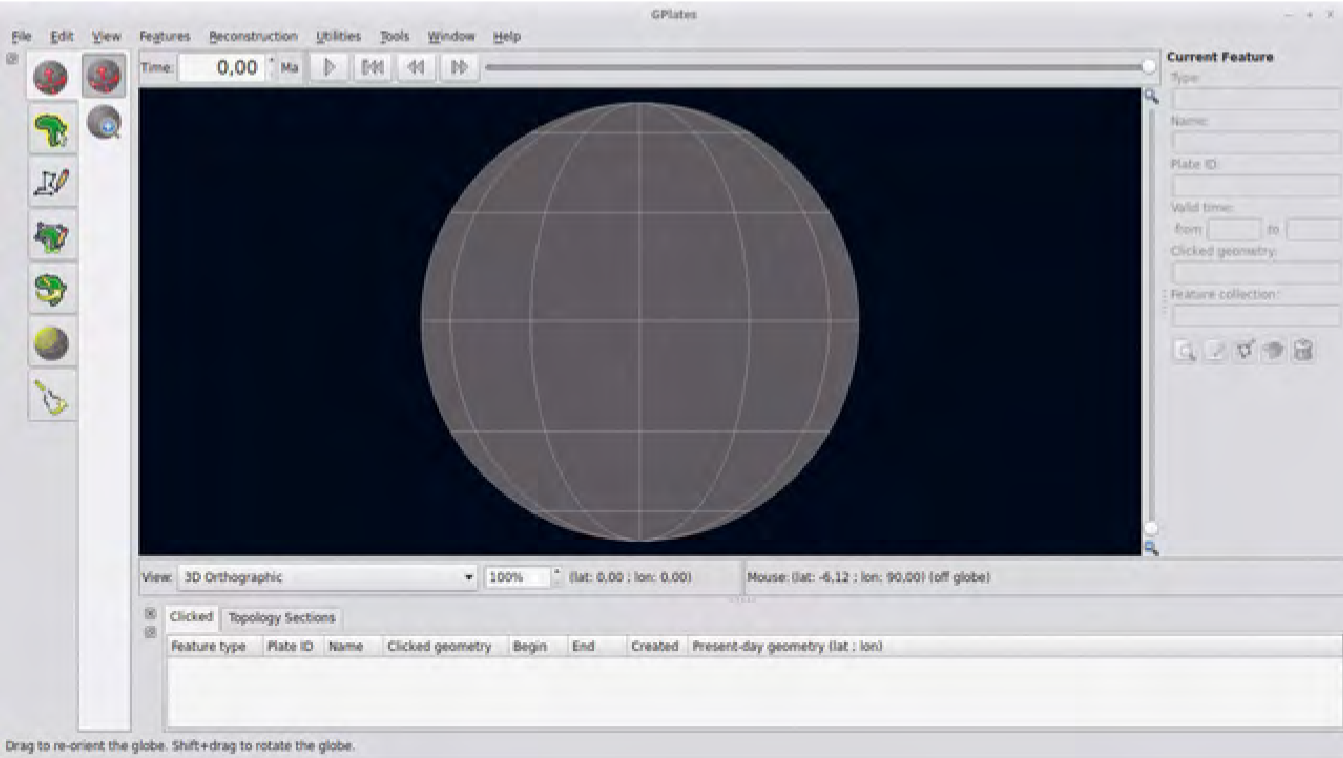
\includegraphics{media/Gplates_interface.png}
\caption{Figure from the We have always been Gephackers chapter, which
they caption ``Gplates interface before loading geodata (grey
earth)''}\label{fig:grey}
}
\end{figure}

Bringing these insights back to their critique of debugging. In this
emerging practises that don't try to``isolate'' these huge and complex
issues so that they are squeezable within hegemonic logics of debugging.
Instead try to feel out and validate situated, nuanced and ephemeral
critiques that can't be reproducible for a developer or for a rigorous
study. This is where they encourage me\footnote{``We need a
  cross-platform, intersoftware, intracommunity, transgenealogical way
  of reporting that, instead of making bugs smaller, scales them up in
  time and space and that can merge untested displacements and
  intersections into its versioning ladder.''(Pritchard, Rocha, and
  Snelting 2021, 250)} to be disobedient to these norms and instead of
scaling down bugs, try to practice them across scales of time and space,
displacing and intersecting the iterations and versions across software
development.

Much like Ahmed's relating to lesbian roles of butch-femme as
performances and not determined roles that I cover in
\href{../../01_Disability_justice_and_life_affirmation_flipping_the_table/sections/01.01.02_Queering_the_axis.md}{01.01.02\_Queering\_the\_axis},
being disobedient doesn't aim to reject or discredit fields of
expertise, practices, scales and knowledges that it works with but to
trouble their performances and problematize their aftermath. This
orients these disobedient actions, so I aim to feel their frictions and
to question how technical systems are imagined, executed and orientated,
moving to figure out how I (and others) can imagine and practise with
them otherwise. Intersecting here with a crip set of
political/relational scales, this refuses access and equality through
assimilation or prescribed terms, but instead makes room to locally
image sets of demands and actions to make. Here I reflect to Collin
Kennedy, who is mentioned in the \emph{Crip Techniscience Manifesto},
and I touched upon earlier in
\href{../../01_Disability_justice_and_life_affirmation_flipping_the_table/sections/01.02.04_Cripping_Technoscience.md}{01.02.04\_Cripping\_Technoscience},.
His refusal to pay to park, and access his care is radically out of the
bugs an access form is imagined to hold, but also questions time,
relational access, and capitalised care.

The Gplates debugging in We Have Always Been Geohackers (ibid) is only
one of a number that they have taken on. These later impositions through
their organisation \emph{The Institute for Technology in the Public
Interest} (TITiPI) and with many collaborators. Through these instances
they are practising disobedience to the norms of big tech's expansive
and violent development. They inquire into how they can gain purchase
and get to grips with what they have capacity to change through
challenging the sedimentations of norms and taking direct action to
re-orient them now. Other examples of these intersections take place on
github where through these disobedient terms of action research they
enthusiastically are ``always-already entangled''(Barad 2007). With
``The long tail of contact tracing''(Aouragh, Pritchard, and Snelting
2020b; 2020a) they pose some of these ``Hardest Problems'' to contact
tracing technologies during the Covid pandemic and their norms towards
surveillance methods and discrimination on the DP-3T (Decentralised
Privacy - Preserving Proximity Tracing ) documents repository. In the
DP-3T repo\footnote{Repo or repository, is a place for storing code,
  files and resources, which is organised through a varying set of
  version control and management protocols that enable the owner to
  manage a stable up to date version of its content.}, as a place
already somewhat critical of the hegemonic centralised norms of other
contact tracing algorithms, welcomed these critiques and conversations,
and these direct provocations evoked dialogue within that development
community. Other repos did not respond in a similar way.

In \emph{EU Digital COVID Certificates: When governments move fast and
break things} (Aouragh et al.~2021b; 2021a) a critique of the EU DCC
(Digital Covid Certificate), this was not the same case. Their
commentary in the issue post/bug report was that a new idtoken which
tracks each person's COVID status and (dis/en)ables them travel and
move, as being something that we should be very cautious of. This is
especially the case when there are no safeguards around who can read and
use the data stored in the QR codes. This is also doubled by the fact
that many of the medical infrastructures in Europe are not fully
digitised, and this approach enforces them to ``scale up'' these
specific digital surveillance systems immediately to comply. They point
out that such quick move to restrictive measures through digital
surveillance infrastructures will undoubtedly hit many issues, which in
these cases will deeply affect the lives of people ``cared'' for by
these systems. Here the disobedient debugging was not met by the same
sort of reception as on the DP-3T post, but instead was within a day
commented on\footnote{``As this is not a technical issue with the
  specification, I will move this to the discussion forum.''(Aouragh et
  al.~2021a)} to say it was in the wrong section (a technical forum) for
this type of discussion. As in it was not a squeezable bug they would
accept. It was then immediately closed and moved to a limited discussion
for just private collaborators of the repo.

Another example of disobedience from them is in their bug report of
Frontier Climate (Aouragh et al.~{[}2017{]} 2024a; {[}2017{]} 2024b)
where they critique Big Techs selling of carbon credits and offset as a
means to not reduce, but expand carbon exploration and dependency. This
debugging showed a different face than the rest, as Frontier totally
deleted the post. This move to delete, instead of the normative
sideline, close down and avoid, shows the power of these comments and
their direct actions to that company. It shows how these critiques if
tabled could potentially reorient things, so have to be thrown off.

These disobedient intersections not only, as said in Pritchard's talk at
4S*EASST (2024), ``give feedback where it is not always wanted'', but in
this direct action of giving feedback to them publicly it shows us how
receptive these organisations and projects are to scaled up bugs. In
their response we can publicly note if they listen and join the
discussion. In this we can also feel them wriggle as they (not so)
subtly restrict the bug to a side room away from discourse. When they
give this feedback and try to get to grips with these scaled up buds, it
is easy to know when they pull away, and into retreat as they delete the
commentary from existence. In these disobedient actions they force the
hand of the repository/software maintainer to not only engage with
political commentary and critiques, but to also position themselves in
relation to it publicly. Do they engage, avoid or squeeze these bugs
however possible? are they too big for them to manage and so they avoid
or do they feel their hold so delete them out of existence? Here I am
thinking of disobedience as a practice to change how dynamics are
performed to show relations, people and bodies under another spectrum,
and to figure out what roles they perform when taken off script.
Reflecting back to
\href{../../01_Disability_justice_and_life_affirmation_flipping_the_table/sections/01.02.04_Cripping_Technoscience.md}{01.02.04\_Cripping\_Technoscience},
these practices align with those of access as friction, and that of the
``non-compliant user'', wiggling room for dialogues where they have been
silenced.

Another key part of this ``giving feedback where it is not always
wanted'' is that of making room for and building up this feedback that
is not wanted. It is about collectively telling other stories of
technologies, infrastructures and policies, than the rhetoric of their
management. Here we can turn to TITiPI and friends work on infrables
(2022), where they present methods for building up bugs from embodied
and experienced relations of infrastructure. These methods not only
build from those of first-person action research but also follow on from
a crip orienting from the sites of impact of infrastructure and politics
to inform the change needed. The work of infrables takes these processes
on by developing a collaborative workshop and practice to unfold these
other stories of Big Tech infrastructures. In this workshop practising
ways to perform and transform anecdotes of infrastructures and their
institutions into fables that can challenge those of mainstream and
dominant narratives.

Bringing this into crip centred methods, I turn to the work of Nat
Decker and Cielo Saucedo's \emph{Cripping\_Computer\_Graphics} (2023).
Here they similarly offer up how cripping as method makes wiggle room
for crip bodies within 3D environments, as well as wider relations and
norms of computation institutions. Here taking up Dr.~Carrie Sandahl
terming of ``cripping'' (2003, 37) as method to make room to feel the
disorientations of crip bodies in relations to the norms of these
technologies. Here they question how the diversity and many
intersections of crip bodies disorient the normalised forms and
mechanics of computer graphics, from the avatars to the ways they are
rigged, and even how these virtual bodies are licensed and sold. Here
they again make room for their crip expertise to question the sedimented
bodies and limits of these systems.

As I shared in the last two chapters the dominant terms are ones of
silencing disabled and frictious voices to keep the narrative straight
and to rule out any queries. By making room to tell these counter
stories, and disobediently performing them as fables, this work aims to
disorient how infrastructures and their aftermaths are felt and
understood through centring the expertise and knowledges of the
communities they are in touch with. These impact centred method are
where I bring in these embodied elements of action research, of working
with crip practitioner knowledge to animate the lines that are drawn and
what is naturalised and sedimented as the norm.

\hypertarget{bringing-disobedience-into-action}{%
\subsubsection{Bringing disobedience into
action}\label{bringing-disobedience-into-action}}

When it comes to bringing these disobedient methods into my Action
Research, I am informed by TITiPI's questioning of the roles and
relations we play when debugging systems. In this thinking about the
scales, relations and capacities we need to make room for the
communities, technologies and change we desire right now. This
disobedience intersecting with the crip cyborg (Kafer 2013), and the
health rebel (Kafer 2017), engaging with and stepping out of line from
the violent norms of computational systems and institutional logics. In
doing this I am also turning to see how these practices of forming
counter narratives, figures and manifestings of sociotechnical fables
can be brought into action in the making of collective infrastructures.
Asking how can my collaborators and I imagine other ways of relating
with these technologies in retreat from their violent origins and
contemporary uses and towards manifesting our own imaginaries and
politics around them.

With a queer disobedience I also take actions through transdisciplinary
approaches which echo Ahmed's wiggle room (2014) loosening of determined
roles to performances. In this wiggling making room with this
disobedience for the roles and discipline within research, forming queer
lines between them. Here I aim to perform these disciplines with respect
and to high quality but along my own lines that subvert the ones they
were prescribed to as isolated institutional discipline.

Disobedience has also been taken along inward arcs of action and into my
internal enquiry and practice. I do this to think through how I can
orient my inquiry by being in touch with the relations I am entangled in
as a crip and queer researcher. This has taken the work mentioned in the
\href{../../00_Introduction/sections/00.01_Background.md}{00.01\_Background}
of the introduction to this research, being individually focused and
technologically centred practice, to now being disorient by collective
bodies and practices that orients the social of infrastructure, with the
assistance of technical. Taking up disobedient action research made room
for me to desist from engaging in what felt like assimilation practices
of computing, to then move to persist with other ways of imagining crip
capacities for care, coalition and interdependence.

Throughout the research there is a returning to a disobedient motion.
This can be read in the
\href{../../02_Crip-Tic_of_Vignettes/02_Crip-Tic_of_Vignettes.md}{02\_Crip-Tic\_of\_Vignettes}
with experiences of surviving institutions through refusal. There is
also disobedience in my work of
\href{../../04_Configure-able_Methods/04_Configure-Able\%20Methods.md}{04\_Configure-Able
Methods} and the forming of a critical access informed approach to the
configuration organisations and infrastructure. These disobedient crip
methods centres points of impact and frictions to figure out localised
interdependent ways towards infrastructural relations. These disobedient
methods are also taken into the two later inquiries of
\href{../../05_In-Configure-Ability/05_In-configure-ability.md}{05\_In-configure-ability}
and
\href{../../06_A\%20Cozier\%20Configure-Ability/06_A\%20Cozier\%20Configure-Ability.md}{06\_A
Cozier Configure-Ability}, where I explore them in action with different
collaborators. This disobedience is also overflowing from this research
in the ways the
\href{../../08_Conclusion/08_Conclusion.md}{08\_Conclusion} covers, of
how these methods are already unfolding into future projects and
infrastructures made with and for communities through disobedient
intersectional queer feminist and crip practices of manifesting action
now.

\hypertarget{bringing-disobedience-into-action-1}{%
\subsubsection{Bringing Disobedience Into
Action}\label{bringing-disobedience-into-action-1}}

When it comes to bringing these disobedient methods into my Action
Research, I am informed by TITiPI's questioning of the roles and
relations we play when debugging systems. In this thinking about the
scales, relations and capacities we need to make room for the
communities, technologies and change we desire right now. This
disobedience intersecting with the crip cyborg (Kafer 2013), and the
health rebel (Kafer 2017), engaging with and stepping out of line from
the violent norms of computational systems and institutional logics. In
doing this I am also turning to see how these practices of forming
counter narratives, figures and manifestings of sociotechnical fables
can be brought into action in the making of collective infrastructures.
Asking how can my collaborators and I imagine other ways of relating
with these technologies in retreat from their violent origins and
contemporary uses and towards manifesting our own imaginaries and
politics around them.

With a queer disobedience I also take actions through transdisciplinary
approaches which echo Ahmed's wiggle room (2014) loosening of determined
roles to performances. In this wiggling making room with this
disobedience for the roles and discipline within research, forming queer
lines between them. Here I aim to perform these disciplines with respect
and to high quality but along my own lines that subvert the ones they
were prescribed to as isolated institutional discipline.

Disobedience has also been taken along inward arcs of action and into my
internal enquiry and practice. I do this to think through how I can
orient my inquiry by being in touch with the relations I am entangled in
as a crip and queer researcher. This has taken the work mentioned in the
\href{../../00_Introduction/sections/00.01.00_Background.md}{00.01.00\_Background}
of the introduction to this research, being individually focused and
technologically centred practice, to now being disorient by collective
bodies and practices that orients the social of infrastructure, with the
assistance of technical. Taking up disobedient action research made room
for me to desist from engaging in what felt like assimilation practices
of computing, to then move to persist with other ways of imagining crip
capacities for care, coalition and interdependence.

Throughout the research there is a returning to a disobedient motion.
This can be read in the
\href{../../02_Crip-Tic_of_Vignettes/02_Crip-Tic_of_Vignettes.md}{02\_Crip-Tic\_of\_Vignettes}
with experiences of surviving institutions through refusal. There is
also disobedience in my work of
\href{../../04_Configure-able_Methods/04_Configure-Able\%20Methods.md}{04\_Configure-Able
Methods} and the forming of a critical access informed approach to the
configuration organisations and infrastructure. These disobedient crip
methods centres points of impact and frictions to figure out localised
interdependent ways towards collective infrastructural relations. These
disobedient methods are also taken into the two later inquiries of
\href{../../05_In-Configure-Ability/05_In-Configure-Ability.md}{05\_In-Configure-Ability}
and
\href{../../06_A\%20Cozier\%20Configure-Ability/06_A\%20Cozier\%20Configure-Ability.md}{06\_A
Cozier Configure-Ability}, where I explore them in action with different
collaborators. This disobedience is also overflowing from this research
in the ways the
\href{../../08_Conclusion/08_Conclusion.md}{08\_Conclusion} covers, of
how these methods are already unfolding into future projects and
infrastructures made with and for communities through disobedient
intersectional queer feminist and crip practices of manifesting action
now.

\hypertarget{inquiring-into-inquiry}{%
\subsection{Inquiring into inquiry}\label{inquiring-into-inquiry}}

This title pulls from a heading of the same name in Living Life as
Inquiry (2021, 445) where Gearty and Marshall undertake inquiry into how
LLI has been undertaken in the prior 20 years since its conception. Here
similarly I am presenting a pair of my inquiries into how I have been
imagining my inquiring. These are presented as two textures and a
figuring out through process and code that made room for me to
conceptualise how these cycles of Action Research could and were
undertaken. The first is from early on in my research, and is an
animation focusing on action research as a cyclical process that emerges
at other places through a building up of cycles. The second from later
on where I was formulating more clearly this disobedient orientation to
action research and taking the form of music visuals from collective and
interactive poem writing, that is dynamically diagrammed into ever
folding and interdependent loops, cycles and rhythms.

\hypertarget{texture-1}{%
\subsubsection{Texture 1}\label{texture-1}}

\begin{figure}
\hypertarget{fig:cyclez}{%
\centering
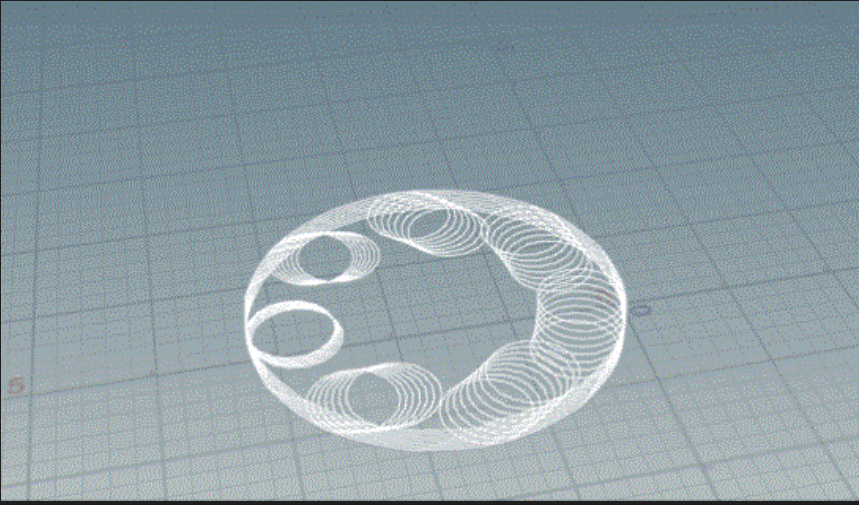
\includegraphics{media/Clyclez.png}
\caption{A still from an animation I made where loops for internal and
external cycles emerging and weaving forms of
research}\label{fig:cyclez}
}
\end{figure}

At the beginning of this PhD I made this animation to reflect on how I
was imagining Action Research as a method that would take me through
loops of inner and outer arcs, ones that will build up, offset and
emerge other forms of inquiry. Looking back at this animation the cycles
presented imagine them as quite linear and deterministic. The form these
cycles build up into are also somewhat walled in, hiding the inner arcs
and sub-cycles of process. This texture gave me grip to get going, and
has through inquiry emerged itself into the
\href{03.04.02_Texture_2.md}{03.04.02\_Texture\_2}. This cycle got
jolted open into these disobedient forms below through an inner arc of
engagement with crip theory that emerged a desire to engage more deeply
with those I am in coalition with as well as making what actions are and
can be reachable through other disobedient practices. What can be
unravelled and made barrier free.

\hypertarget{texture-2}{%
\subsubsection{Texture 2}\label{texture-2}}

\begin{figure}
\hypertarget{fig:loops}{%
\centering
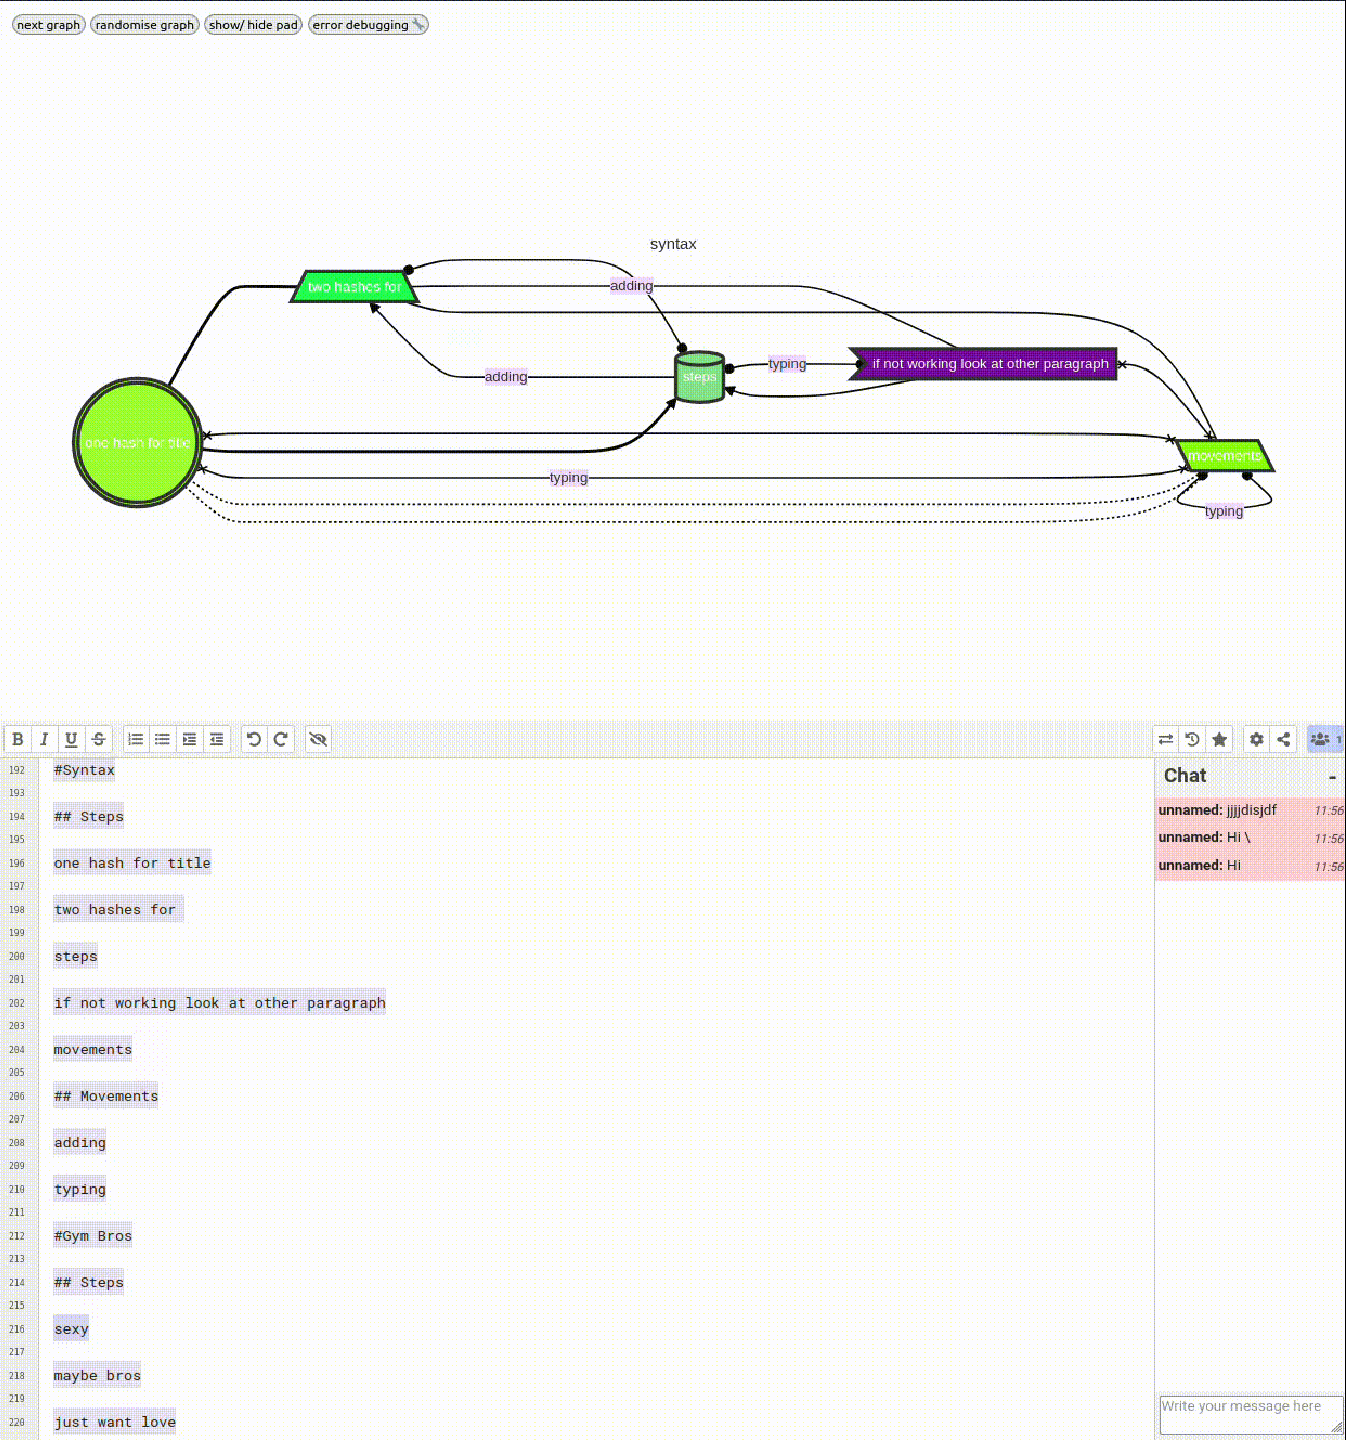
\includegraphics{media/Pad_Loop.png}
\caption{A screenshot of the work generating looped diagrams (top) from
the collective etherpad (bellow)}\label{fig:loops}
}
\end{figure}

This texture and artwork came about as I was trying to reflectively
figure out how these disobedient actions had taken place. This texture
takes the form of a poem visualiser that pulls from collective written
texts in an etherpad and dynamically produces complex and indeterminate
diagrams with a multiplicity of paths and connections between the
lines/nodes of the poem (\cref{fig:loops}). It is also made to be audio
reactive so it can generate diagrams in-sync to music as visuals. This
work was produced in collaboration with Sunni Liao and Yewen Jin
(members of In-grid\footnote{In-grid is a Trans*Feminist collective who
  I helped to set up and work with throughout this research.}) for an
event called \emph{In-grid.Real\_bodies2.1}\footnote{https://www.in-grid.io/projects/real-bodies-2.1/
  \#\# What was Actioned?} that In-grid held in 2024 at Avalon Cafe and
performed live in collaboration with the audience. The work acting as a
texture in this research opens up the disobedient actions to be less
determinable cycles and into poetic movements, both in content and
connection. It also opens up these actions to be public, to be
intersect-able, barrier free (ish) and accessible, moving from the
isolated static spiral to instead be engulfed in the rhythms of music,
dancing and collective being. Its context has moved from an isolated
animation, and determinable rendering, through to making room for an
accessible, dynamic and pleasurable tool or infrastructure, made with
and for collaboration. In a disobedient move here this methodology
refuses to isolate in this study and instead moves from the shared pad
to the poem to the diagram to the dance floor to the here on the
academic thesis (but also to the *****\footnote{``This chronic job, by
  stating all the cron variables of time as *, refuses such linear
  computational metrics to instead hold the past*present*future,
  future*past*present, and * * * * * of crip times.'' (Simms and
  Marangoni 2025)}).

If you want to try it out, see what's happened there and maybe intersect
into a texture of this methodology you can try it
\href{https://georgie-png.github.io/etherpad-vis/}{HERE}.

When it comes to summing up the actions taken for this project they are
fairly entangled by the ways I have been taking many internal and
external arcs of research through a number of contexts. I have though
found it helpful to map these arcs into three movements, which are
themselves covered by each of the following three chapters. These stages
overlap and have greatly informed one another, as well as many
happenings that do not quite fit into this thesis, but I found this
approach helpful to orient these movements more accessibly. An initial
sense-making stage of inquiry into
\href{../../04_Configure-able_Methods/04_Configure-Able\%20Methods.md}{04\_Configure-Able
Methods} aims to figure out configuration methods by rubbing up against
them and finding frictions with them from my crip axis. Through this I
offer up the disobedient configure-able methods that emerges localised
improvised collective configurations as affirming infrastructural and
institutional re-configuring and hacking practices. I then move to
practise these methods with what is in reach, and orienting towards
collaborating with In-grid to figure out
\href{../../05_In-Configure-Ability/05_In-Configure-Ability.md}{05\_In-Configure-Ability}
as a place to collective orient our sociotechnical systems through
critical access. This made room for us to try to distribute our capacity
to manage and know these relations and in that movement also distribute
the power and expertise in our relations. I also orient to try and put
more disabled futures in reach by manifesting
\href{../../06_A\%20Cozier\%20Configure-Ability/06_A\%20Cozier\%20Configure-Ability.md}{06\_A
Cozier Configure-Ability}, where I emerge a crip network infrastructure
and collaboration that aims to crip and disorient these sociotechnical
infrastructures through bringing with us crip politics of affirmation,
care, access and the indeterminate embodied knowing and expertise of
disabled bodies.

Even though these are presented as distinct sections I want to encourage
an understanding of how these movements have come into being together
with the figure below. These overlapping and overflowing movements to me
represent a disorienting from the prescribed and determined norms, and a
orienting to crip politics, experience, need and desire.

\hypertarget{ethical-considerations}{%
\subsection{Ethical considerations}\label{ethical-considerations}}

In taking on this research and inquiry their of course have been many
ethical relations to address. In my practice of ethics I have also
queried these norms of the institutional forms of ethics, both in the
ways they navigate ethics, but also how they template it for me to fill
in. In this research this had been enacted by doing more traditional
ethics forms for the
\href{../../05_In-Configure-Ability/sections/05.03.02.00_Configure-ability_In-Workshops.md}{05.03.02.00\_Configure-ability\_In-Workshops}
and the
\href{../../05_In-Configure-Ability/sections/05.02_Processing\%20In-Configure-ability.md}{05.02\_Processing
In-Configure-ability} focus groups I have taken on, making sure they
know what the research is, sign to consent, and have the ability to
remove consent. In following these norms of course I have found friction
along my Crip axis. One of places I have found friction is with the
mandatory use of both ZOOM and Outlook, as being the ethical secure
spaces for this research. This is because they are able to ``stably''
provide a service which fits to the tick-box regulations of GDPR, even
with their fluctuating terms (Rob Pegoraro, 2023), and in doing so
secure the stability of institutional contracts. Why I find friction is
that Big tech models and tick-box economies that this research is trying
to wiggle around, and so being forced to use them seems slightly
unethical, and undermining. The unethical aspect also accentuated by the
scales of these cloud economies, of the politics these infrastructures
enforce when you use them, and the inability to orient otherwise in the
inflexible hard systems.

This was particularly true when it came to how to document my working
together with others, both in workshops and focus groups. Here instead
of orienting towards these infrastructures which in many ways reinforce
research as surveillance, where we document exact words in time, hold
people to them and orient arguments from them, I disoriented to forming
collective notes, of taking time to care for what people wanted to say
and to manifesting an inquiry together. This move for me not only
ethically changes how we engage with the communities we work with and
the infrastructures we meet them with, retreating from surveillance
norms, but also as a researcher with fatigue it has reduced my labour
hugely. This reduction in labour also making the research itself more
ethical for me to take, and also opening up critique around what we
might have capacity for in research, if we are not trying to hold these
people and their words in place. It also orients to the critique that
runs throughout this research, that representation and assimilation in
sedimented technologies and their naturalised ethics isn't always that
ethical, and we can find other disobedient ways to disorient these
relations to our own crip and queer axes, desires and needs.

This retreat from a particular type of individualised practise of
research and ethics is highlighted in the way I have been undertaking my
First Person Action Research. Here much like Marshall (Marshall, 2004),
I have initiated focus groups with those I have inquired into working
with. These have been enacted through a-synchronous collective
reflections, based through my drafted inquiries and signal chat
(groups), and where I invited feedback from others and room for them to
add their own perspective. Orienting towards this direction has brought
much joy into this research, as I reflect back with collaborators and
companions on our times together, of how it has emerged into compounding
reflections and unfolding actions. This felt quite vulnerable for me to
do, and I definitely delayed and anxiously avoided it for a while, but
it has also added much more depth to my research and made room for me
reconsider my normalised and sedimented paths toward these inquiries.

\hypertarget{conclusion}{%
\subsection{Conclusion}\label{conclusion}}

In this chapter I have presented the methodology that my research
project has undertaken. As I have shown, it aims to hold together both
the embodied practices and resulting knowledges that the crip and queer
framing I have previously formulated makes room for and embraces. These
methods informed by and developed through disobedient and direct actions
within different collaborations and coalitions.

In reflection of and in tandem with the
\href{../../04_Configure-able_Methods/sections/04.02.00_Inquiring\%20into\%20Critical\%20Access.md}{04.02.00\_Inquiring
into Critical Access}'s two textures evoked earlier, I am pleased with
the ways these actions have unfolded in practice. This has taken my
practice from a place of predominantly isolated technical practise to
one of orienting on the tables of interdependent action and change
within ongoing and emerging groups. This work disobediently follows the
line of AR and ILL to understand these projects and practises as ever
ongoing. I personally find this wiggle room for continuation cozy,
opening up possibilities for how I can collectivley action crip
manifestings within diverse localities which are yet to unfold.
